\documentclass{ximera}

%\usepackage{todonotes}
%\usepackage{mathtools} %% Required for wide table Curl and Greens
%\usepackage{cuted} %% Required for wide table Curl and Greens
\newcommand{\todo}{}

\usepackage{esint} % for \oiint
\ifxake%%https://math.meta.stackexchange.com/questions/9973/how-do-you-render-a-closed-surface-double-integral
\renewcommand{\oiint}{{\large\bigcirc}\kern-1.56em\iint}
\fi


\graphicspath{
  {./}
  {ximeraTutorial/}
  {basicPhilosophy/}
  {functionsOfSeveralVariables/}
  {normalVectors/}
  {lagrangeMultipliers/}
  {vectorFields/}
  {greensTheorem/}
  {shapeOfThingsToCome/}
  {dotProducts/}
  {partialDerivativesAndTheGradientVector/}
  {../productAndQuotientRules/exercises/}
  {../normalVectors/exercisesParametricPlots/}
  {../continuityOfFunctionsOfSeveralVariables/exercises/}
  {../partialDerivativesAndTheGradientVector/exercises/}
  {../directionalDerivativeAndChainRule/exercises/}
  {../commonCoordinates/exercisesCylindricalCoordinates/}
  {../commonCoordinates/exercisesSphericalCoordinates/}
  {../greensTheorem/exercisesCurlAndLineIntegrals/}
  {../greensTheorem/exercisesDivergenceAndLineIntegrals/}
  {../shapeOfThingsToCome/exercisesDivergenceTheorem/}
  {../greensTheorem/}
  {../shapeOfThingsToCome/}
  {../separableDifferentialEquations/exercises/}
  {vectorFields/}
}

\newcommand{\mooculus}{\textsf{\textbf{MOOC}\textnormal{\textsf{ULUS}}}}

\usepackage{tkz-euclide}\usepackage{tikz}
\usepackage{tikz-cd}
\usetikzlibrary{arrows}
\tikzset{>=stealth,commutative diagrams/.cd,
  arrow style=tikz,diagrams={>=stealth}} %% cool arrow head
\tikzset{shorten <>/.style={ shorten >=#1, shorten <=#1 } } %% allows shorter vectors

\usetikzlibrary{backgrounds} %% for boxes around graphs
\usetikzlibrary{shapes,positioning}  %% Clouds and stars
\usetikzlibrary{matrix} %% for matrix
\usepgfplotslibrary{polar} %% for polar plots
\usepgfplotslibrary{fillbetween} %% to shade area between curves in TikZ
\usetkzobj{all}
\usepackage[makeroom]{cancel} %% for strike outs
%\usepackage{mathtools} %% for pretty underbrace % Breaks Ximera
%\usepackage{multicol}
\usepackage{pgffor} %% required for integral for loops



%% http://tex.stackexchange.com/questions/66490/drawing-a-tikz-arc-specifying-the-center
%% Draws beach ball
\tikzset{pics/carc/.style args={#1:#2:#3}{code={\draw[pic actions] (#1:#3) arc(#1:#2:#3);}}}



\usepackage{array}
\setlength{\extrarowheight}{+.1cm}
\newdimen\digitwidth
\settowidth\digitwidth{9}
\def\divrule#1#2{
\noalign{\moveright#1\digitwidth
\vbox{\hrule width#2\digitwidth}}}





\newcommand{\RR}{\mathbb R}
\newcommand{\R}{\mathbb R}
\newcommand{\N}{\mathbb N}
\newcommand{\Z}{\mathbb Z}

\newcommand{\sagemath}{\textsf{SageMath}}


%\renewcommand{\d}{\,d\!}
\renewcommand{\d}{\mathop{}\!d}
\newcommand{\dd}[2][]{\frac{\d #1}{\d #2}}
\newcommand{\pp}[2][]{\frac{\partial #1}{\partial #2}}
\renewcommand{\l}{\ell}
\newcommand{\ddx}{\frac{d}{\d x}}

\newcommand{\zeroOverZero}{\ensuremath{\boldsymbol{\tfrac{0}{0}}}}
\newcommand{\inftyOverInfty}{\ensuremath{\boldsymbol{\tfrac{\infty}{\infty}}}}
\newcommand{\zeroOverInfty}{\ensuremath{\boldsymbol{\tfrac{0}{\infty}}}}
\newcommand{\zeroTimesInfty}{\ensuremath{\small\boldsymbol{0\cdot \infty}}}
\newcommand{\inftyMinusInfty}{\ensuremath{\small\boldsymbol{\infty - \infty}}}
\newcommand{\oneToInfty}{\ensuremath{\boldsymbol{1^\infty}}}
\newcommand{\zeroToZero}{\ensuremath{\boldsymbol{0^0}}}
\newcommand{\inftyToZero}{\ensuremath{\boldsymbol{\infty^0}}}



\newcommand{\numOverZero}{\ensuremath{\boldsymbol{\tfrac{\#}{0}}}}
\newcommand{\dfn}{\textbf}
%\newcommand{\unit}{\,\mathrm}
\newcommand{\unit}{\mathop{}\!\mathrm}
\newcommand{\eval}[1]{\bigg[ #1 \bigg]}
\newcommand{\seq}[1]{\left( #1 \right)}
\renewcommand{\epsilon}{\varepsilon}
\renewcommand{\phi}{\varphi}


\renewcommand{\iff}{\Leftrightarrow}

\DeclareMathOperator{\arccot}{arccot}
\DeclareMathOperator{\arcsec}{arcsec}
\DeclareMathOperator{\arccsc}{arccsc}
\DeclareMathOperator{\si}{Si}
\DeclareMathOperator{\scal}{scal}
\DeclareMathOperator{\sign}{sign}


%% \newcommand{\tightoverset}[2]{% for arrow vec
%%   \mathop{#2}\limits^{\vbox to -.5ex{\kern-0.75ex\hbox{$#1$}\vss}}}
\newcommand{\arrowvec}[1]{{\overset{\rightharpoonup}{#1}}}
%\renewcommand{\vec}[1]{\arrowvec{\mathbf{#1}}}
\renewcommand{\vec}[1]{{\overset{\boldsymbol{\rightharpoonup}}{\mathbf{#1}}}\hspace{0in}}

\newcommand{\point}[1]{\left(#1\right)} %this allows \vector{ to be changed to \vector{ with a quick find and replace
\newcommand{\pt}[1]{\mathbf{#1}} %this allows \vec{ to be changed to \vec{ with a quick find and replace
\newcommand{\Lim}[2]{\lim_{\point{#1} \to \point{#2}}} %Bart, I changed this to point since I want to use it.  It runs through both of the exercise and exerciseE files in limits section, which is why it was in each document to start with.

\DeclareMathOperator{\proj}{\mathbf{proj}}
\newcommand{\veci}{{\boldsymbol{\hat{\imath}}}}
\newcommand{\vecj}{{\boldsymbol{\hat{\jmath}}}}
\newcommand{\veck}{{\boldsymbol{\hat{k}}}}
\newcommand{\vecl}{\vec{\boldsymbol{\l}}}
\newcommand{\uvec}[1]{\mathbf{\hat{#1}}}
\newcommand{\utan}{\mathbf{\hat{t}}}
\newcommand{\unormal}{\mathbf{\hat{n}}}
\newcommand{\ubinormal}{\mathbf{\hat{b}}}

\newcommand{\dotp}{\bullet}
\newcommand{\cross}{\boldsymbol\times}
\newcommand{\grad}{\boldsymbol\nabla}
\newcommand{\divergence}{\grad\dotp}
\newcommand{\curl}{\grad\cross}
%\DeclareMathOperator{\divergence}{divergence}
%\DeclareMathOperator{\curl}[1]{\grad\cross #1}
\newcommand{\lto}{\mathop{\longrightarrow\,}\limits}

\renewcommand{\bar}{\overline}

\colorlet{textColor}{black}
\colorlet{background}{white}
\colorlet{penColor}{blue!50!black} % Color of a curve in a plot
\colorlet{penColor2}{red!50!black}% Color of a curve in a plot
\colorlet{penColor3}{red!50!blue} % Color of a curve in a plot
\colorlet{penColor4}{green!50!black} % Color of a curve in a plot
\colorlet{penColor5}{orange!80!black} % Color of a curve in a plot
\colorlet{penColor6}{yellow!70!black} % Color of a curve in a plot
\colorlet{fill1}{penColor!20} % Color of fill in a plot
\colorlet{fill2}{penColor2!20} % Color of fill in a plot
\colorlet{fillp}{fill1} % Color of positive area
\colorlet{filln}{penColor2!20} % Color of negative area
\colorlet{fill3}{penColor3!20} % Fill
\colorlet{fill4}{penColor4!20} % Fill
\colorlet{fill5}{penColor5!20} % Fill
\colorlet{gridColor}{gray!50} % Color of grid in a plot

\newcommand{\surfaceColor}{violet}
\newcommand{\surfaceColorTwo}{redyellow}
\newcommand{\sliceColor}{greenyellow}




\pgfmathdeclarefunction{gauss}{2}{% gives gaussian
  \pgfmathparse{1/(#2*sqrt(2*pi))*exp(-((x-#1)^2)/(2*#2^2))}%
}


%%%%%%%%%%%%%
%% Vectors
%%%%%%%%%%%%%

%% Simple horiz vectors
\renewcommand{\vector}[1]{\left\langle #1\right\rangle}


%% %% Complex Horiz Vectors with angle brackets
%% \makeatletter
%% \renewcommand{\vector}[2][ , ]{\left\langle%
%%   \def\nextitem{\def\nextitem{#1}}%
%%   \@for \el:=#2\do{\nextitem\el}\right\rangle%
%% }
%% \makeatother

%% %% Vertical Vectors
%% \def\vector#1{\begin{bmatrix}\vecListA#1,,\end{bmatrix}}
%% \def\vecListA#1,{\if,#1,\else #1\cr \expandafter \vecListA \fi}

%%%%%%%%%%%%%
%% End of vectors
%%%%%%%%%%%%%

%\newcommand{\fullwidth}{}
%\newcommand{\normalwidth}{}



%% makes a snazzy t-chart for evaluating functions
%\newenvironment{tchart}{\rowcolors{2}{}{background!90!textColor}\array}{\endarray}

%%This is to help with formatting on future title pages.
\newenvironment{sectionOutcomes}{}{}



%% Flowchart stuff
%\tikzstyle{startstop} = [rectangle, rounded corners, minimum width=3cm, minimum height=1cm,text centered, draw=black]
%\tikzstyle{question} = [rectangle, minimum width=3cm, minimum height=1cm, text centered, draw=black]
%\tikzstyle{decision} = [trapezium, trapezium left angle=70, trapezium right angle=110, minimum width=3cm, minimum height=1cm, text centered, draw=black]
%\tikzstyle{question} = [rectangle, rounded corners, minimum width=3cm, minimum height=1cm,text centered, draw=black]
%\tikzstyle{process} = [rectangle, minimum width=3cm, minimum height=1cm, text centered, draw=black]
%\tikzstyle{decision} = [trapezium, trapezium left angle=70, trapezium right angle=110, minimum width=3cm, minimum height=1cm, text centered, draw=black]


\outcome{State and use Stokes' theorem.}

\title[Dig-In:]{Stokes' theorem}

\begin{document}
\begin{abstract}
  We introduce Stokes' theorem.
\end{abstract}
\maketitle

Our final fundamental theorem of calculus is Stokes'
theorem. Historically speaking, Stokes' theorem was discovered after
both Green's theorem and the divergence theorem. Its application is
probably the most obscure, with the primary applications being rooted
in electricity-and-magnetism and fluid dynamics.

Nevertheless, once we know Stokes' theorem, we can view it as a direct
generalization of Green's theorem.

\begin{theorem}[Stokes' Theorem]\index{Stokes' Theorem}
  If the components of $\vec{F}:\R^3\to\R^3$ have continuous partial
  derivatives and $\partial R$ is a boundary of a closed surface $R$
  and $\vec{p}(t)$ parameterizes $\partial R$ in a counterclockwise
  direction with the interior on the left, then:
  \[
  \iint_R (\curl \vec{F})\dotp \uvec{n}\d S = \oint_{\partial R}
  \vec{F}\dotp\d\vec{p}
  \]
\end{theorem}

If we compare the conclusion of Stokes' theorem to the conclusion of
Green's theorem, we see that they are quite similar:
  \[
  \underbrace{\iint_R \curl\vec{F}\d A = \oint_{\partial R} \vec{F}\dotp\d\vec{p}}_{\text{Green's Theorem}}\qquad \underbrace{\iint_R (\curl \vec{F})\dotp \uvec{n}\d S = \oint_{\partial R}
  \vec{F}\dotp\d\vec{p}}_{\text{Stokes' Theorem}}
  \]
  Like Green's theorem, Stokes' theorem compute circulation along a surface:
  \begin{image}
    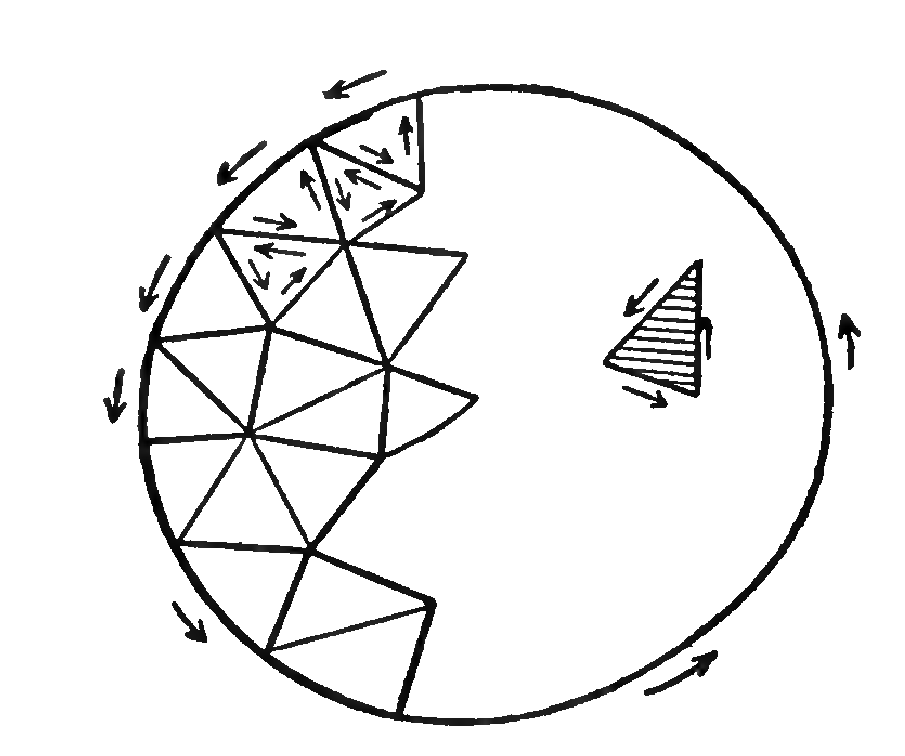
\includegraphics{circulation.png}
  \end{image}
  In essence, Green's theorem is nothing more than Stokes' theorem
  when we assume that the surface is restricted to the $(x,y)$-plane.


\section{Transforming integrals}

Like the divergence theorem, one application of Stokes' theorem is to
transform a difficult integral into an easier one.

\begin{example}
  Consider the line integral
  \[
  \oint_C (x-y)\d x +(x-2y+z) \d y + (3x+z) \d z
  \]
  where $C$ is parameterized by $\vec{p}(t) =
  \vector{\cos(t),\sin(t),3}$, $0\le t<2\pi$. Compute this integral
  using Stokes' theorem.
  \begin{explanation}
    Let $R$ be the surface bounded by $C$, so in this case $C =
    \partial R$. Moreover, set
    \[
    \vec{F}(x,y,z) = \vector{x-y,x-2y+z,3x+z}.
    \]
    Now we may write:
    \[
    \oint_C (x-y)\d x +(x-2y+z) \d y + (3x+z) \d z = \oint_{\partial R} \vec{F}\dotp\d\vec{p} 
    \]
    and Stokes' theorem says:
    \[
    \oint_{\partial R} \vec{F}\dotp\d\vec{p}  = \iint_R (\curl \vec{F})\dotp \uvec{n}\d S
    \]
    Write with me,
    \begin{align*}
      \curl F(x,y,z) = \vector{\answer[given]{-1},\answer[given]{-3},\answer[given]{2}}\\
      \uvec{n} = \vector{\answer[given]{0},\answer[given]{0},\answer[given]{1}}.
    \end{align*}
    Hence
    \[
    \iint_R \vector{-1,-3,2}\dotp \vector{0,0,1}\d S = \answer[given]{2}\iint_R \d S
    \]
    but
    \[
    \iint_R \d S = \answer[given]{\pi}
    \]
    Hence
    \[
    \oint_C (x-y)\d x +(x-2y+z) \d y + (3x+z) \d z =\answer[given]{2\pi}.
    \]
  \end{explanation}
\end{example}


%% \section{Observations from Stokes' theorem}
%% Explain how to change the surface
%% fact that circulation on any closed surface is zero.
%% In particular, if the boundry is contained to a plane, the avg value of the surface normals is exactly the normal vector to the plane

\section{Swapping surfaces}

Since Stokes' theorem says that if we want to evaluate the circulation
along a surface, we need only look at the boundary, we can sometimes
be very clever, and swap one surface for another, provided that they
have the \textit{same} boundary! Consider the pictures below:

\begin{image}
  \begin{tikzpicture}
    \draw[gray,ultra thick] plot[smooth] coordinates {(-1.5,1.5) (-1,3) (0,3.3)  (1.5,1.5)};
    \shade[ball color=white!50!gray] plot[smooth] coordinates {(-1.5,1.5) (-1,3) (0,3.3)  (1.5,1.5)};
    \shade[top color=black!50!gray, middle color=black]  (0,1.5) ellipse (1.5 and .3);
    \draw[black,ultra thick] (0,1.5) ellipse (1.5 and .3);
    
    \node[inner sep=0pt] at (0,0) {$\iint_R (\curl\vec{F})\dotp \uvec{n}\d S$};

    \node[inner sep=0pt] at (2.1,0) {$=$};
    
    \draw[black,ultra thick] (4,1.5) ellipse (1.5 and .3);
    \node[inner sep=0pt] at (4,0) {$\oint_{\partial R = \partial D} \vec{F}\dotp\d \vec{p}$};

    \node[inner sep=0pt] at (5.9,0) {$=$};
    
    \draw[black,ultra thick,fill=white!50!gray] (8,1.5) ellipse (1.5 and .3);
    \node[inner sep=0pt] at (8,0) {$\iint_D (\curl\vec{F})\dotp \uvec{n}\d S$};

  \end{tikzpicture}
\end{image}

Above we see a region $R$ on the left and a region $D$ on the
right. In the middle is the boundary of \textit{both} regions. Since
both regions $R$ and $D$ have the same boundary, we can effectively
\textit{swap} surfaces by using Stokes' Theorem. Check out the next
example.


\begin{example}
  Consider the surface integral
  \[
  \iint_R (\curl \vec{F})\dotp \uvec{n}\d S
  \]
  where
  \[
  \vec{F}(x,y,z) = \vector{-y,0,z^2}
  \]
  and $R$ is the upper hemisphere of the sphere:
  \[
  x^2 + y^2 + z^2 = 9
  \]
  Compute this integral using Stokes' theorem.
  \begin{explanation}
    Note that the boundary of the sphere is \textbf{identical} to the boundary of the disk
    \[
    \vec{p}(t) = \vector{3\cos(t),3\sin(t),0}
    \]
    where $0\le t<2\pi$. Hence we may dispense with our ``upper
    hemisphere'' and simply work with the disk of radius $3$.
    Write with me,
    \[
    \curl F(x,y,z) = \vector{\answer[given]{0},\answer[given]{0},\answer[given]{1}}
    \]
    Hence
    \begin{align*}
      \iint_R \vector{0,0,1}\dotp \vector{0,0,1}\d S &= \iint_R \d S\\
      &=\answer[given]{9\pi}.
    \end{align*}
    By Stokes' theorem this is equal to the integral we desire.
  \end{explanation}
\end{example}




\section{Our final fundamental theorem of calculus}

How is Stokes' Theorem a fundamental theorem of calculus? Well
consider this:
\begin{image}
  \begin{tikzpicture}
    \draw[gray,ultra thick] plot[smooth] coordinates {(-1.5,1.5) (-1,3) (0,3.3)  (1.5,1.5)};
    \shade[ball color=white!50!gray] plot[smooth] coordinates {(-1.5,1.5) (-1,3) (0,3.3)  (1.5,1.5)};
    \shade[top color=black!50!gray, middle color=black]  (0,1.5) ellipse (1.5 and .3);
    \draw[black,ultra thick] (0,1.5) ellipse (1.5 and .3);
    
    \node[inner sep=0pt] at (0,0) {$\iint_R (\curl\vec{F})\dotp \uvec{n}\d S\quad =\quad \oint_{\partial R} \vec{F}\dotp\d\vec{p}$};

    \node at (-1.5,-.7) {$\underbrace{\hspace{8.5em}}$};

    \node at (2,-.7) {$\underbrace{\hspace{5em}}$};

    \node[below,inner sep=0pt,text width=5cm,scale=.5] at (-1.3,-1)
         {To compute the circulation along a surface $R\subseteq\R^3$, };

    \node[below,inner sep=0pt,text width=4cm,scale=.5] at (2.2,-1) {we can compute the accumulation of $\vec{F}$ along a boundary curve $\partial R$.};
  \end{tikzpicture}
\end{image}


Are there no more fundamental theorems of calculus? Well, there are,
but as you will see if you continue your study of mathematics, they
are all generalizations of the theorems we already know.


For some interesting extra reading check out:
\begin{itemize}
\item \link[\textit{The History of Stokes' Theorem}, V.J.\ Katz,
  Mathematics Magazine, May
  1979.]{http://www.jstor.org/stable/2690275}
\end{itemize}

\end{document}
